\begin{enumerate}
	\item \textbf{Deactivate Voter}
		\begin{enumerate}
			\item \textbf{Service Contract}
				\begin{figure}[H]
					\centering
					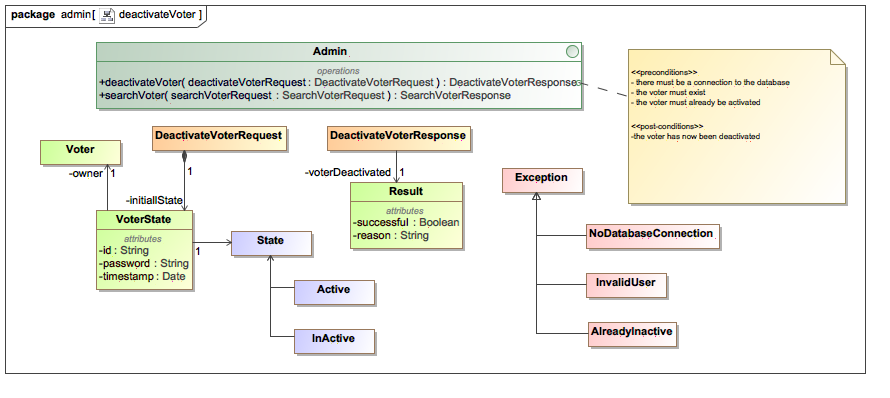
\includegraphics[width=0.75\linewidth]{../Images/Admin/ServiceContracts/deactivateVoter_ServiceContract.png}
					\caption{Deactivate Voter Service Contract}
				\end{figure}
				
				Deactivate Voter requires an ID number in the request which will be used to change the ActiveState state to inactive if all pre-conditions are met.
				\newline	
								
				\begin{enumerate}
					\item Pre-conditions
					\begin{itemize}
						\item There must be a connection to the database
						\item The voter must exist
						\item the voter must already be activated
					\end{itemize}
					
					\item Exceptions
					\begin{itemize}
						\item If there is no connection to the database, the NoDatabaseConnection exception will be thrown
						\item If a voter's ID is not valid, the IdDoesNotExist exception will be thrown
						\item If the voter is already active, the AlreadyActive exception will be thrown
					\end{itemize}
					
					\item Post-conditions
					\begin{itemize}
						\item The voter is now deactivated
					\end{itemize}
				\end{enumerate}
			
			\newpage\textsl{}
			
			\item \textbf{Functional Requirements}
				\begin{figure}[H]
					\centering
					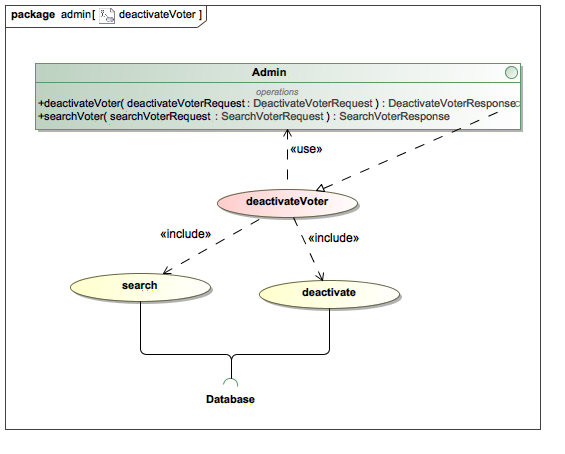
\includegraphics[width=0.75\linewidth]{../Images/Admin/UseCases/deactivateVoter_useCase.png}
					\caption{Deactivate Voter Use Case}
				\end{figure}
				
				The Deactivate Voter process will call the DeactivateVoter use case from the database module.
				\newline
				
			\item \textbf{Process Design}
				\begin{figure}[H]
					\centering
					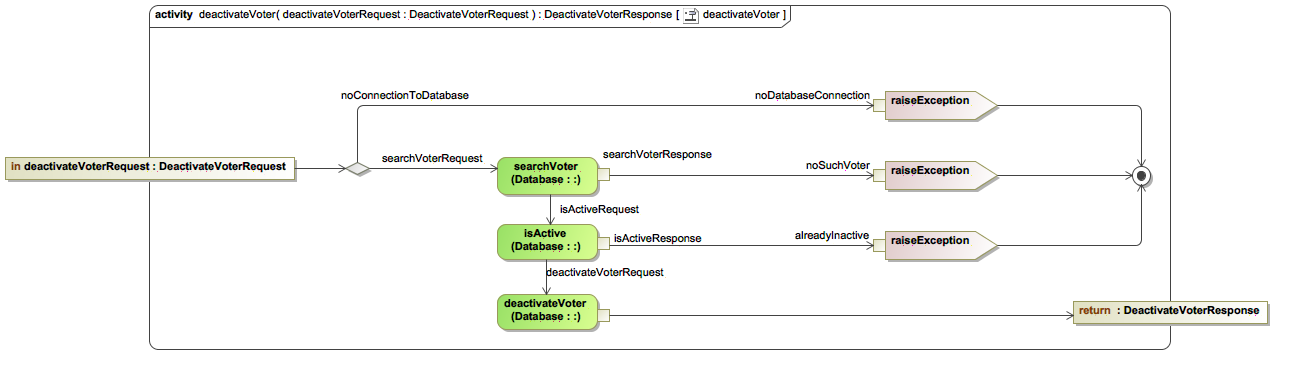
\includegraphics[width=0.75\linewidth]{../Images/Admin/ActivityDiagrams/deactivateVoter_ActivityDiagram.png}
					\caption{Deactivate Voter Activity}
				\end{figure}
				
				The Deactivate Voter process will first retrieve the ID number from the request and validate if is a valid ID number, after which it will get all the necessary Voter details from the database which corresponds to that ID number. It then checks in what state the voter is to see if it has already been deactivated. If all cases are valid, then the voter's ActiveState will change from Valid to Invalid.
				\newline
				
		\end{enumerate}
		
		\newpage
\end{enumerate}